\chapter{Hadoop}
\label{chap:Hadoop}

Hadoop started in 2006 based on Google's work of GFS (now is called HDFS -
Sect.\ref{sec:HadoopFS}) and MapReduce. Nowadays, Hadoop 2.x is much bigger with
many more components (Sect.\ref{sec:MR1_MR2}).

\section{Why Hadoop was developed?}

Big data is not just big in terms of bytes, but also type (e.g., a single hard
disk likely contains relations, text, images, and spreadsheets) and structure
(e.g., a large corpus of relational databases may have millions of unique
schemas). As a result, certain long-held assumptions --- e.g., that the database
schema is always known before writing a query --- are no longer useful guides
for building data management systems.

Hadoop has emerged from a solution for large-scale web-crawling and indexing
engine to a general-purpose computing platform for the next-generation of
data-based applications. 

Hadoop uses two-step disk-based MapReduce implementation on Hadoop HDFS. To
enable using data on HDFS for other tasks, e.g. machine learning where iterative
algorithms are often used, there are several packages have been developed:
Apache Spark (Sect.\ref{sec:apache_spark}).

\subsection{Hadoop is NOT}

\begin{itemize}
  \item ESB
  \item NoSQL
  \item HPC
  \item Relational 
  \item Real-time
\end{itemize}

Data is added into the HDFS system, but you cannot ask Hadoop to return a list
of all the data matching a specific data set. 
The primary reason for this is that Hadoop doesn't store, structure, or
understand the structure of the data that is being stored within HDFS. One
soltuion is to use HBase (a distributed database system on top of HDFS). 

\subsection{Key Hadoop data types}

The below types of data are widely added to HDFS (Sect.\ref{sec:HadoopFS})
\begin{itemize}
  \item Sentiment
  \item Clickstream
  \item Sensor/Machine
  \item Geographic
  \item Server logs
  \item Text
\end{itemize}


\section{Critics of Hadoop}

It was designed to run on-premises in data centers with the advantage of using
low-cost machines.
But now everyone is moving to cloud. Y

\begin{enumerate}
  \item ou can run Hadoop in the cloud. But it is not cost effective.

  \item  Hadoop is getting fatter with so different components.
  
  Today, the architecture picture
  of Hadoop looks like a zoo hosting HDFS, YARN, MapReduce, Tez, Pig, Hive,
  Impala, Kudu, HBase, Accumulo, Flume, Sqoop, Falcon, Samza, etc.
  
  Because original Hadoop (with only HDFS and MapReduce) is not good enough to
  meet customer's demands, the community has developed a lot of new tools into
  the Hadoop ecosystem over the years.
  
  This is rational and necessary to win the competition. However, it also
  inevitably reaches the status of overshooting. 
  
  
 Rarely customers need all of them. If no need, why bother running a full blown
 Hadoop cluster? So, options to pick only needed components such as
 \begin{itemize}
   \item  Parquet + Spark
   
   \item Apache Samza, a stream processing engine that was originally designed
   on top of Hadoop YARN
   
   Netflix has recently contributed the feature of static partition assignments
   that allows Samza to be used without YARN. This cool feature enables Netflix
   to run Samza applications in AWS EC2 instances without any Hadoop/YARN
   dependency.
 \end{itemize}
  
  \item HBase, the NoSQL engine of Hadoop, is not as competitive as other noSQL
  solutions.
  
  Compared to other popular NoSQL solutions such as MongoDB and Cassandra, HBase
  has a lot of functionality and unique features. It also has battle proven
  scalability and availability.
  Moreover, Apache Trafodion, built on top of HBase, even provides fully ACID
  SQL. However, it is only ranked at 15 on DB-Engines Ranking, way behind
  MongoDB and Cassandra. The biggest reason that HBase is left behind is that
  Hadoop distributors' marketing commitment to HBase has never risen to nearly
  the level of MongoDB's or DataStax's push behind their respective core
  products.
  
  Technically, HBase is also more complicated to setup and operate because of
  the dependency to other Hadoop services.
  
  \item Spark, Kafka, Mesos, Docker, etc. are better than their counterparts of
  Hadoop or fill in blank space. And they get endorsements from heavy weights
  like IBM. 
\end{enumerate}
\url{https://haifengl.wordpress.com/2016/03/03/the-future-of-hadoop-is-misty/}


\section{Hadoop distributors}

Apache Hadoop is the main open-source repository for Hadoop development. Other
than that, there are 3 main Hadoop distributions, target to commercial licenses
\begin{enumerate}
  \item Cloudera CDH: plan to provide ``enterprise datahub'', i.e. there is no
  need for datawarehouse at company
  
  It has free version and commercial version. Some features are not open-source.
  
  \item Hortonwork Hadoop: this is the 100\% open-source distribution, and the
  main driver for Hadoop development at Apache, e.g. YARN module.
  
  \item MapR Hadoop: this one does not use HDFS, but use MapRFS (a proprietary
  distributed file system). 
  
  The free version is MapR's M3 Edition. It provides proprietary modules to ease
  the maintenance and usage of a Hadoop system at companies which do not have
  programmers/experts in Hadoop.
\end{enumerate}
All of these products are rooted from Apache Hadoop.

\section{Apache Hadoop}

A Hadoop cluster is a special type of computational cluster designed
specifically for storing and analyzing huge amounts of unstructured data in a
distributed computing environment. As of early 2013, Facebook was recognized as
having the largest Hadoop cluster in the world. Other prominent users include
Google, Yahoo and IBM. These clusters use Hadoop framework. 

Hadoop has its origin from Apache Nutch (Sect.\ref{sec:Nutch}).
The 2 components in Nutch were applicable beyond the realm of search, and thus
an independent project was created in Feb, 2006 called Hadoop. Then Doug Cutting
joined Yahoo, and help to turn Hadoop into a system that ran at web scale, e.g.
10,000-core Hadoop cluster. In Jan, 2008, Apache Hadoop become the top-level
project. 

In April 2008, Hadoop broke a world record to become the fastest system to sort
a terabyte of data. Running on a 910-node cluster, Hadoop sorted one terabyte in
209 seconds (just under $3^\frac{1}{2}$ minutes), beating the previous year's winner
of 297 seconds. In November of the same year, Google reported that its MapReduce
implementation sorted one terabyte in 68 seconds. Then a team at
Yahoo! used Hadoop to sort one terabyte in 62 seconds.

Hadoop framework is written in Java that enables running a Java app on large
clusters of commodity hardware (i.e. low costs) as it's running on a single
machine. Hadoop's HDFS is the distributed file system (Sect.\ref{sec:HadoopFS}).
It should be installed in a cluster. However, we can deploy on a single machine
by configuring a pseudo-distributed single-node Hadoop cluster.

The project's creator, Doug Cutting, explains how the name came about:
\begin{verbatim}
The name my kid gave a stuffed yellow elephant. Short, relatively easy to spell
and pronounce, meaningless, and not used elsewhere: those are my naming
criteria. Kids are good at generating such. Googol is a kid's term.  
\end{verbatim} 
Subprojects and ``contrib" modules in Hadoop also tend to have names that are
unrelated to their function, often with an elephant or other animal theme
(``Pig," for example). Smaller components are given more descriptive (and
therefore more mundane) names. This is a good principle, as it means you can
generally work out what something does from its name. For example, the
jobtracker keeps track of MapReduce jobs.    

Hadoop Ecosystem, which includes all of the additional software packages that
can be installed on top of or alongside Hadoop, such as Apache Hive, Apache Pig
and Apache Spark. Hadoop is Consistent and partition tolerant, i.e. it falls
under the CP category of the CAP theoram.
\begin{enumerate}
  \item Hadoop Common
  \item Hadoop HDFS:
  \item Hadoop YARN (added from Hadoop 2.0):  resource-management platform
  responsible for managing compute resources in clusters and using them for scheduling of users' applications.
  \item Hadoop MapReduce: a programming model for large scale data processing.
\end{enumerate}

\subsection{Hadoop computing engine}
\label{sec:hadoop_node_structure}

For processing the data, the Hadoop Map/Reduce ships code (typically Java-code
.jar file) to to the nodes that have the required data, and the nodes then
process the data in parallel. So, each node functions as ``data'' source and
computing unit which takes advantage of data locality. \textcolor{red}{This is
in contrast to HPC architecture which split data cluster and compute cluster,
but connect through high-speed networking}. 

Although Java code is common, any programming language can be used with "Hadoop
Streaming" to implement the "map" and "reduce" parts of the user's program. To
expose higher level APIs, Apache Pig, Apache Hive and Apache Spark have been
added. 
\url{http://en.wikipedia.org/wiki/Apache_Hadoop}

Next, you need to know the structure of a Hadoop cluster. 
A small Hadoop cluster includes a single master (which functions as both
NameNode and JobTracker) and multiple worker nodes.
The master node can function as a JobTracker (Resource Manager), TaskTracker
(NodeManager), NameNode and DataNode.
A slave or worker node acts as both a DataNode and TaskTracker, though it is
possible to have data-only worker nodes and compute-only worker nodes. NOTE:
TaskTracker are compute-node.

\begin{enumerate}
  \item one machine as NameNode, one machine as Resource Manager (or aka
  JobTracker).
    
  These machines are the masters.
  \begin{itemize}
    \item NameNode stores HDFS filesystem information in a file named
    \verb!fsimage!. Updates to the file system (add/remove blocks) are not
    updating the fsimage file, but instead are logged into a file, so the I/O
    is fast append only streaming as opposed to random file writes. Only when
    restaring, before it can serve client requests, the namenode reads the
    fsimage and then applies all the changes from the log file to bring the filesystem state up to date in
    memory (a new fsimage consisting of the prior fsimage plus the application
    of all operations from the edit logs). It remains in safe mode until a
    sufficient number of blocks have been reported by datanodes. This process
    takes time. Administrators typically access the NameNode web UI at the first
    sign of trouble.  Unfortunately, the NameNode wouldn't start its HTTP server
    until after writing a new checkpoint.  In a slow startup situation, it could
    take multiple minutes or even more than an hour after restarting the
    NameNode before the web UI would be accessible which makes it would appear
    as though the NameNode process had hung during startup.
    Only an experienced Hadoop operator would be able to determine that the
    NameNode is in fact making progress, by using relatively low-level
    techniques such as inspecting thread dumps.
    \footnote{\url{http://hortonworks.com/blog/understanding-namenode-startup-operations-in-hdfs/}}
    
    Since Hadoop 2.0, a new feature called Secondary NameNode added. What it
    does is to help boosting the start-up time; not as a full replicate of the
    NamaNode.\footnote{\url{http://stackoverflow.com/questions/19970461/name-node-vs-secondary-name-node}}
    
    
  \end{itemize}
  
  \item The rest of the machines: act as both DataNode and NodeManager
  (TaskTracker).
  
  All these machines depend on the NameNode. If the name node falls the cluster
  goes down.
  
  \item (optional) one machine as Secondary NameNode: this machine does not
  function as a seconday to the NameNode machine. Instead,  it periodically read
  the filesystem changes log and apply them into the fsimage file, thus bringing
  the fsimage file up to date so that the NameNode start up faster next time.
  No slaves can connect to the Secondary NameNode; so if the NameNode is down,
  the whole Hadoop cluster still fails.
  
\end{enumerate}
In a larger cluster, the HDFS is managed through a dedicated NameNode server to
host the file system index, and a Secondary NameNode that can generate snapshots
of the namenode's memory structures, thus preventing file-system corruption and
reducing loss of data. Similarly, a standalone JobTracker server (Resource
Manager) can manage job scheduling.


Your MapReduce jobs may be IO bound or CPU/Memory bound -if you know which one
is more important (effectively how many CPU cycles/RAM MB used per Map or
Reduce), you can make better decisions. 


\subsection{Hadoop YARN}
\label{sec:YARN}

Yarn has been added to Hadoop 2.0. 
With YARN, you can now run multiple applications in Hadoop, all sharing a common
resource management.  As of September, 2014, YARN manages only CPU (number of
cores) and memory, but management of other resources such as disk, network
and GPU is planned for the future.



\subsection{User authentication and authorization}

Hadoop doesn't do any authentication of users. This is an important realization
to make, because it can have serious implications in a corporate data center.
The NameNode and the JobTracker don't require any authentication.
Hadoop has the ability to require authentication, in the form of Kerberos
principals (Sect.\ref{sec:Kerberos}). 

Hadoop can use the Kerberos protocol to ensure that when someone
makes a request, they really are who they say they are. This mechanism is used
throughout the cluster. In a secure Hadoop configuration, all of the Hadoop
daemons use Kerberos to perform mutual authentication, which means that when two
daemons talk to each other, they each make sure that the other daemon is who it
says it is. Additionally, this allows the NameNode and JobTracker to ensure that
any HDFS or MR requests are being executed with the appropriate authorization
level.

HDFS implement a permission model much like POSIX model. Each file and directory
is associated with an owner and a group. The file or directory has separate
permissions for the user that is the owner, for other users that are members of
the group, and for all other users.  The difference from POSIX:
\begin{verbatim}
In contrast to the POSIX model, there are no setuid or setgid bits for files as
there is no notion of executable files.

For directories, there are no setuid or setgid bits directory as a
simplification..

The Sticky bit can be set on directories, preventing anyone except the
superuser, directory owner or file owner from deleting or moving the files
within the directory. Setting the sticky bit for a file has no effect.
\end{verbatim}

In the context of MapReduce, the users and groups are used to determine who is
allowed to submit or modify jobs. In MapReduce, jobs are submitted via queues
controlled by the scheduler.
Administrators can define who is allowed to submit jobs to particular queues via
MapReduce ACLs (Access Control Lists).  


The downside to doing this is that if that user and group really don't exist, no
one will be able to access that file except the superusers, which, by default,
includes hdfs, mapred, and other members of the hadoop supergroup.  


% \section{Experiences with Hadoop}
% 

\subsection{Configure environment: hadoop-env.sh}
\label{sec:hadoop-env.sh}

Administrators should use the conf/hadoop-env.sh script to do site-specific
customization of the Hadoop daemons' process environment.

The file
\begin{verbatim}
/usr/local/hadoop/etc/hadoop/hadoop-env.sh
\end{verbatim}
control the path to java, and the setting for the four different
daemons NameNode/DataNode and JobTracker/TaskTracker. Each daemon receives
configuration options specified in the associated environment variable, which
maps to
\begin{verbatim}
NameNode           	HADOOP_NAMENODE_OPTS
DataNode            HADOOP_DATANODE_OPTS
SecondaryNameNode   HADOOP_SECONDARYNAMENODE_OPTS
JobTracker          HADOOP_JOBTRACKER_OPTS
TaskTracker         HADOOP_TASKTRACKER_OPTS
\end{verbatim}
%different locations which contaisn files that Hadoop needs to use, and the
% different system settings, e.g. maximum heap size

As Hadoop is used to run Java applications (hadoop daemons), these settings are
designed to control how a Java MapReduce applications run and use resources
\begin{verbatim}
JAVA_HOME
HADOOP_OPTS (extra args to java-runtime, default:  
            -Djava.net.preferIPv4Stack=true)

HADOOP_CONF_DIR

JSVC_HOME

HADOOP_CLASSPATH

# max heap to use
HADOOP_HEAPSIZE (in MB, default:1000)
HADOOP_NAMENODE_INIT_HEAPSIZE (in MB, default: 1000)

## 
HADOOP_NAMENODE_OPTS
  "-Dhadoop.security.logger=${HADOOP_SECURITY_LOGGER:-INFO,RFAS}
  -Dhdfs.audit.logger=${HDFS_AUDIT_LOGGER:-INFO,NullAppender} $HADOOP_NAMENODE_OPTS"
HADOOP_DATANODE_OPTS
  "-Dhadoop.security.logger=ERROR,RFAS $HADOOP_DATANODE_OPTS"
HADOOP_SECONDARYNAMENODE_OPTS

HADOOP_NFS3_OPTS
HADOOP_PORTMAP_OPTS (default: -Xmx512m)

## apply to commands such as: fs, dfs, fschk, distcp
HADOOP_CLIENTS_OPTS (default: -Xmx512m)
HADOOP_JAVA_PLATFORM_OPTS


# secure DataNode
HADOOP_SECURE_DN_USER

# location of log file
HADOOP_LOG_DIR (default: $HADOOP_HOME/logs)
          (we can use $HADOOP_LOG_DIR/$USER)
HADOOP_SECURE_DN_LOG_DIR (default: ${HADOOP_LOG_DIR}/${HADOOP_HDFS_USER})


# location of PID file
HADOOP_PID_DIR    (default: /tmp)
        however should be set to a location that is accessible by only the 
        'hadoop' group's users, to avoid potential symlink attack
HADOOP_SECURE_DN_PID_DIR

# a string representation of the instance of hadoop
HADOOP_IDENT_STRING   (default: $USER) 

\end{verbatim}

Example: enable parallelGC  on NameNode daemon
\begin{verbatim}
export HADOOP_NAMENODE_OPTS="-XX:+UseParallelGC ${HADOOP_NAMENODE_OPTS}" 
\end{verbatim}

Example: in a multi-user Hadoop cluster, you may need to configure the log dir
\begin{verbatim}
HADOOP_LOG_DIR
\end{verbatim}

Example: maximum heapsize (in MB) for each daemon (default: 1000MB)
\begin{verbatim}
HADOOP_HEAPSIZE
\end{verbatim}

\section{Changes from Hadoop 1.x to Hadoop 2.x}
\label{sec:MR1_MR2}

Hadoop 1.x basically has 2 components: HDFS and MapReduce.

Hadoop 2.x has revised and break MapReduce down into different projects, each
does a particular job. A new and important layer above HDFS is YARN (batch
processing management) which allows new components to be added (Spark, BSP,
Hama, MapReduce, HBase (database system)) or existing programming models to use
(e.g. MPI). \url{http://www.wiziq.com/blog/hadoop-1-vs-hadoop-2/}

\subsection{Hadoop 1}

\begin{enumerate}
  \item Limited up to 4000-nodes per cluster
  \item The bottleneck is based on the number of tasks in a cluster: O(\# tasks
  in a cluster)
  
  \item JobTracker does multiple things: resource management, job scheduling and
  monitoring $\rightarrow$ which causes the bottleneck
  
  \item Only one namespace for managing HDFS
  \item Map and Reduce slots are static
  \item only job to run is MapReduce.
  
  \item The namespaces for APIs
\begin{verbatim}
org.apache.hadoop.mapreduce.Partitioner
org.apache.hadoop.mapreduce.Mapper
org.apache.hadoop.mapreduce.Reducer
org.apache.hadoop.mapreduce.Job
\end{verbatim} 
\end{enumerate}


\url{http://www.slideshare.net/RommelGarcia2/hadoop-1x-vs-2}

\begin{figure}[hbt]
  \centerline{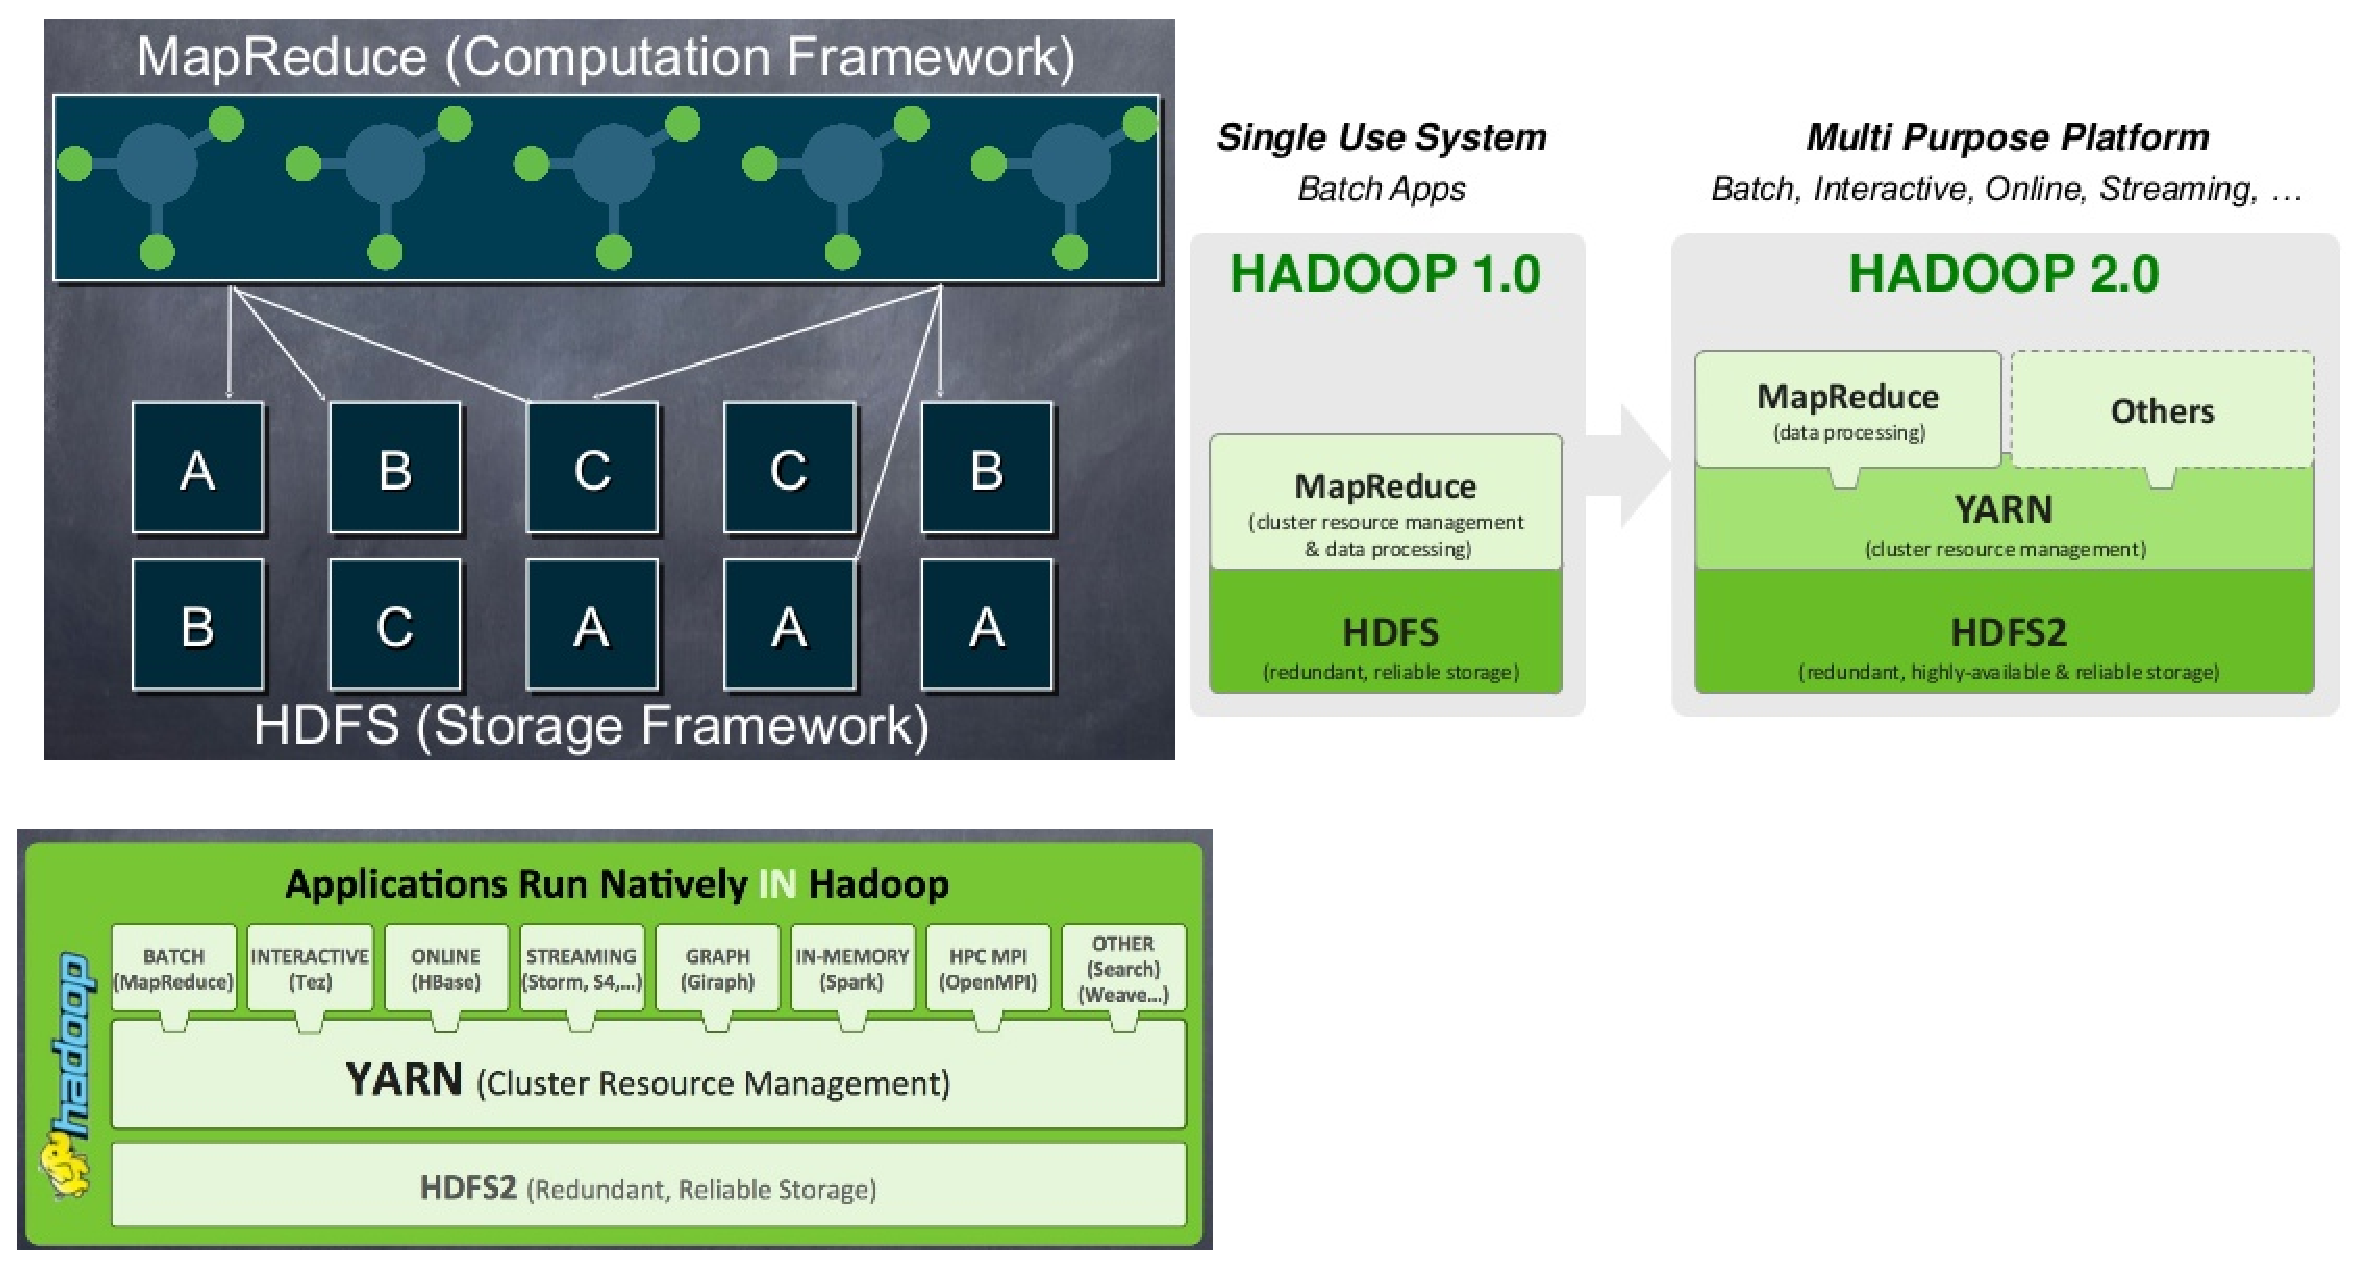
\includegraphics[height=6cm,
    angle=0]{./images/MR1_MR2_comparison_01.eps}}
  \caption{MR1 to MR2}
  \label{fig:MR1_MR2_comparison_01}
\end{figure}


\subsection{Hadoop 2}

backward compatible with MR1
\begin{enumerate}
  \item Support upto to 10,000 nodes per cluster
  \item The bottleneck is based on the cluster size: O(cluster size)
  \item The function of JobTracker in MR1 is different in MR2. To avoid
  scaling issues, JobTracker is splitted into different components, each with
  its specialized purpose (see below). Resource manager is carried out by the new component: YARN.
  
  \item multiple namespace for managing HDFS, Fig.\ref{fig:MR1_MR2_comparison_02}
  \item YARN is used as Resource Manager.
\begin{verbatim}
org.apache.hadoop.yarn.api.ApplicationClientProtocol
org.apache.hadoop.yarn.api.ApplicationMasterProtocol
org.apache.hadoop.yarn.api.ContainerManagementProtocol
\end{verbatim}  
  
  \item HDFS support multiple storage tiers: Disk, Memory, SSD
  
  \item any job can be integrated with Hadoop
  \item support other languages (not only Java)
\end{enumerate}
\url{http://www.slideshare.net/tshooter/strata-conf2014}

\begin{figure}[hbt]
  \centerline{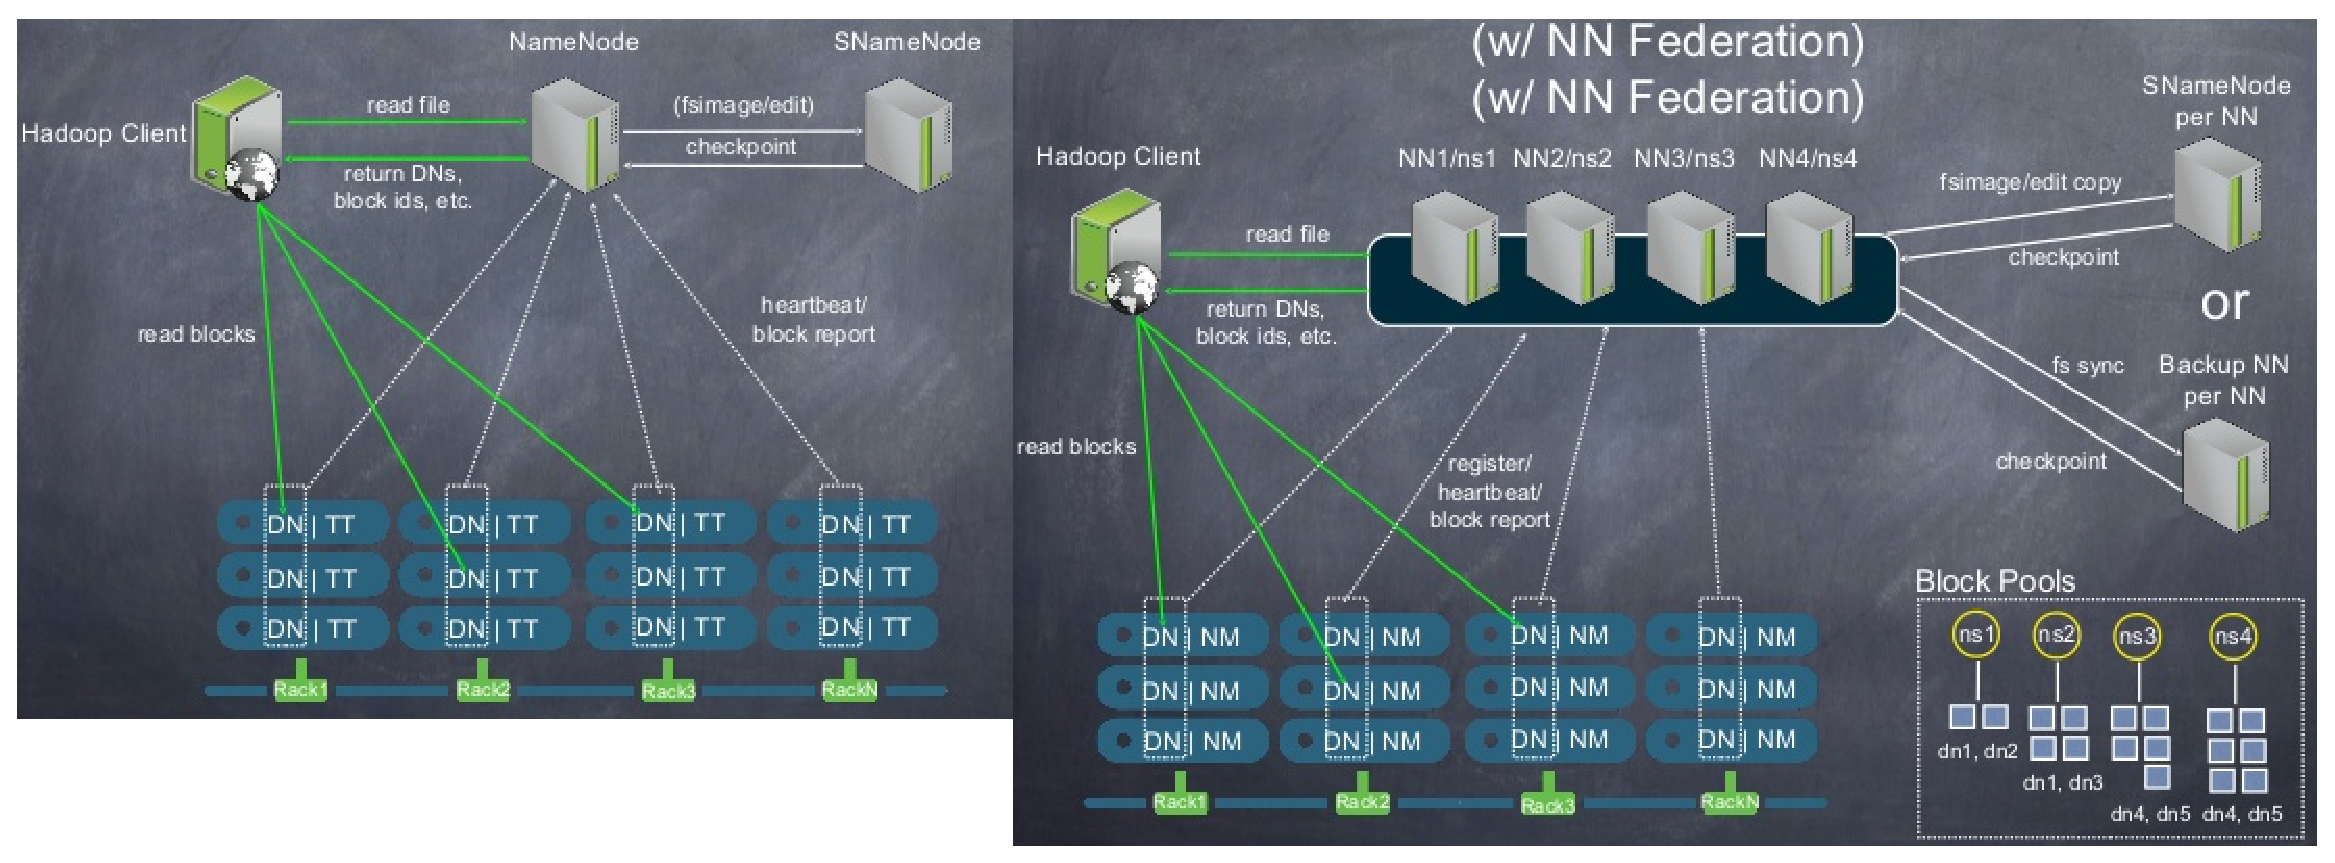
\includegraphics[height=3cm,
    angle=0]{./images/MR1_MR2_comparison_02.eps}}
  \caption{MR1 to MR2 comparison: Data can reside on NameNodes of different
  namespace}
  \label{fig:MR1_MR2_comparison_02}
\end{figure}

The reason is that in Hadoop 2, MapReduce is split into 2
components: the cluster resource management capabilities have become YARN; and
the MapReduce-specific capabilities remain MapReduce. This is known as MR2
architecture; while the old one is called MR1.
\begin{enumerate}
  \item In the former MR1 architecture, the cluster was managed by a service
  called the JobTracker.
  
  \item In MR2 architecture: the functions of the JobTracker are divided into
  three services.
  \begin{itemize}
    \item The ResourceManager is a persistent YARN service that receives and
    runs applications (a MapReduce job is an application) on the cluster
    \item 
  \end{itemize}
\end{enumerate}

\subsection{List of deprecated keys}

\url{https://hadoop.apache.org/docs/r2.2.0/hadoop-project-dist/hadoop-common/DeprecatedProperties.html}

{\small
\begin{verbatim}
[INFO] deprecation - mapred.jar is deprecated. Instead, use mapreduce.job.jar
[INFO] deprecation - mapred.map.child.log.level is deprecated. Instead, use mapreduce.map.log.level
[INFO] deprecation - mapred.reduce.child.log.level is deprecated. Instead, use mapreduce.reduce.log.level
[INFO] deprecation - mapred.output.value.groupfn.class is deprecated. Instead, use mapreduce.job.output.group.comparator.class
[INFO] deprecation - mapred.output.key.comparator.class is deprecated. Instead, use mapreduce.job.output.key.comparator.class
[INFO] deprecation - mapred.cache.files is deprecated. Instead, use mapreduce.job.cache.files
[INFO] deprecation - mapred.mapoutput.key.class is deprecated. Instead, use mapreduce.map.output.key.class
[INFO] deprecation - mapreduce.inputformat.class is deprecated. Instead, use mapreduce.job.inputformat.class
[INFO] deprecation - mapreduce.partitioner.class is deprecated. Instead, use mapreduce.job.partitioner.class
[INFO] deprecation - mapred.job.name is deprecated. Instead, use mapreduce.job.name
[INFO] deprecation - mapred.mapoutput.value.class is deprecated. Instead, use mapreduce.map.output.value.class
[INFO] deprecation - mapred.job.tracker is deprecated. Instead, use mapreduce.jobtracker.address
[INFO] deprecation - fs.default.name is deprecated. Instead, use fs.defaultFS
[INFO] deprecation - mapred.local.dir is deprecated. Instead, use mapreduce.cluster.local.dir
[INFO] deprecation - fs.checkpoint.edits.dir is deprecated. Instead, use dfs.namenode.checkpoint.edits.dir
[INFO] deprecation - dfs.data.dir is deprecated. Instead, use dfs.datanode.data.dir
[INFO] deprecation - fs.checkpoint.dir is deprecated. Instead, use dfs.namenode.checkpoint.dir
[INFO] deprecation - mapred.temp.dir is deprecated. Instead, use mapreduce.cluster.temp.dir
[INFO] deprecation - dfs.name.dir is deprecated. Instead, use dfs.namenode.name.dir
[INFO] deprecation - mapred.system.dir is deprecated. Instead, use mapreduce.jobtracker.system.dir
[INFO] deprecation - fs.default.name is deprecated. Instead, use fs.defaultFS
[INFO] deprecation - mapreduce.map.class is deprecated. Instead, use mapreduce.job.map.class
[INFO] deprecation - dfs.name.edits.dir is deprecated. Instead, use dfs.namenode.edits.dir
[INFO] deprecation - user.name is deprecated. Instead, use mapreduce.job.user.name
[INFO] deprecation - mapred.cache.files.filesizes is deprecated. Instead, use mapreduce.job.cache.files.filesizes
[INFO] deprecation - fs.default.name is deprecated. Instead, use fs.defaultFS
[INFO] deprecation - mapred.reduce.tasks is deprecated. Instead, use mapreduce.job.reduces
[INFO] deprecation - mapreduce.reduce.class is deprecated. Instead, use mapreduce.job.reduce.class
[INFO] deprecation - mapred.output.dir is deprecated. Instead, use mapreduce.output.fileoutputformat.outputdir
[INFO] deprecation - mapred.map.tasks is deprecated. Instead, use mapreduce.job.maps
[INFO] deprecation - mapred.cache.files.timestamps is deprecated. Instead, use mapreduce.job.cache.files.timestamps
[INFO] deprecation - mapred.working.dir is deprecated. Instead, use mapreduce.job.working.dir
\end{verbatim}
}
\url{https://groups.google.com/forum/#!msg/scoobi-dev/OiWMwnxpoQE/H4fjQBMF3vcJ}
\section{Resource in Hadoop}
\label{sec:Hadoop_resources}

A resource is an XML-based file that contain a set of name/value pair.

\subsection{Read-only configuration}

These files contains the read-only configuration
\begin{verbatim}
src/core/core-default.xml 
src/hdfs/hdfs-default.xml 
src/mapred/mapred-default.xml.
\end{verbatim}
It comes with some default settings. 


By default, Hadoop has 2 resources, loaded in the order they are specified
in the classpath
\begin{verbatim}
core-default.xml   # read-only information
core-site.xml      # site-specific information (for a given Hadoop installation)
\end{verbatim}

The configuration in the form
\begin{verbatim}
<property>
    <name>property-name</name>
    <value>property-value</value>

  </property>
\end{verbatim}

Example: specify 
\begin{verbatim}
<property>
  <name>dfs.datanode.data.dir</name>
  <value>file:///usr/local/hadoop/data/datanode</value>
  <description>DataNode directory</description>
</property
\end{verbatim}
we can declare a key/value pair as {\it final} (i.e. no subsequently-loaded
resource can modify the value). Typically, the {\it final} key/value pair are
stored in \verb!core-site.xml! file so that user application cannot alter.
\begin{verbatim}
<property>
    <name>dfs.client.buffer.dir</name>
    <value>/tmp/hadoop/dfs/client</value>
    <final>true</final>
  </property>
\end{verbatim}


There are so many pre-defined names from Hadoop. From your application, you can
modify these key/value pair by loading the classpath
\begin{verbatim}
java.lang.Object
    org.apache.hadoop.conf.Configuration
\end{verbatim}
with the predefined methods to handle the modification of them.
\url{http://hadoop.apache.org/docs/r1.2.1/api/org/apache/hadoop/conf/Configuration.html}

\subsection{Site-specific configuration}

These are files that contains configuration that you can modify and it is
site-specific, i.e. it can be different from one machine to another.
\begin{verbatim}
conf/core-site.xml
conf/hdfs-site.xml 
conf/mapred-site.xml
\end{verbatim}

You can control the Hadoop scripts found in the bin/ directory of the
distribution, by setting site-specific values via the conf/hadoop-env.sh
(Sect.\ref{sec:hadoop-env.sh}).

\subsection{core-site.xml}
\label{sec:core-site.xml}

The URI to the NodeName can be defined in the key \verb!fs.defaultFS! (the
deprecated key (since Hadoop 2.0) is fs.default.name)
\url{https://issues.apache.org/jira/browse/AMBARI-2789}


\subsection{yarn-site.xml}
\label{sec:yarn-site.xml}

We need to specify the machine that functions as the ResourceTracker
\begin{verbatim}
<property>
<name>yarn.resourcemanager.resource-tracker.address</name>
<value>10.10.10.104:8025</value>
</property>
<property>
\end{verbatim}

Then we choose what shuffle process to handle the 
\begin{verbatim}
<property>
   <name>yarn.nodemanager.aux-services</name>
   <value>mapreduce_shuffle</value>
</property>
<property>
   <name>yarn.nodemanager.aux-services.mapreduce_shuffle.class</name>
   <value>org.apache.hadoop.mapred.ShuffleHandler</value>
</property>
\end{verbatim}
\url{https://developer.yahoo.com/hadoop/tutorial/module1.html}

\section{Disk configuration}

\url{http://cloud-dba-journey.blogspot.com/2013/08/hadoop-reference-architectures.html}

Hadoop is quite different than other services in conventional data centers, such
as web, mail, and database servers. They are learning that to achieve optimal
performance, you need to pay particular attention to configuring the underlying
hardware.
\url{http://hortonworks.com/blog/proper-care-and-feeding-of-drives-in-a-hadoop-cluster-a-conversation-with-stackiqs-dr-bruno/}

Having lots of disks per server gives you more raw IO bandwidth than having one
or two big disks. If you have enough that different tasks can be using different
disks for input and output, disk seeking is minimized, which is one of the big
disk performance killers. That said: more disks have a higher power budget; if
you are power limited, you may want fewer but larger disks.    

\subsection{Ext3 or Ext4 or XFS or btrfs or zfs}

\textcolor{red}{Don't use LVM; it adds latency and causes a bottleneck.}  

\begin{enumerate}
  \item XFS: internally it uses B+ trees and Extends to store data. It is fully
  supported in Ubuntu. \url{https://wiki.ubuntu.com/XFS}
  \item Ext3/Ext4: use H trees
\end{enumerate}

Yahoo! has publicly stated they use ext3. Regardless of the merits of the
filesystem, that means that HDFS-on-ext3 has been publicly tested at a bigger
scale than any other underlying filesystem that we know of.


Ext4 has better performance with large files. However, the Ext4 Linux filesystem
has delayed allocation of data which makes it handle unplanned server
shutdowns/power outages less well than classic ext3. Consider turning off the
delalloc option in /etc/fstab unless you trust your UPS.

XFS offers better disk space utilization than ext3 and has much quicker disk
formatting times than ext3. This means that it is quicker to get started with a
data node using XFS. However, most often, the limitation is not disk-read, but 
I/O and RAM limitations will be more important. XFS is not included in basic
RedHat Enterprise Linux.


So, \textcolor{red}{ext3 is the most common choice.} However, since Ubuntu
12.04, the preferred one is XFS, EXT4, EXT3 in that order.

Create one single partition
\begin{verbatim}
fdisk /dev/sdb
\end{verbatim}
Format the partition with EXT4
\begin{verbatim}
mkfs.ext4 /dev/sdb1
\end{verbatim}

Automount to /data/0, /data/1 (if we have more disk)
by modifying /etc/fstab file
\begin{verbatim}	
/dev/sdb1  /data/0  ext4   defaults,noatime,nodiratime
      1    2
\end{verbatim}
NOTE: We use these as we don't need these information and thus can improve disk
performance
\begin{verbatim}
noatime = skip writing file access time to disk
          everytime a file is accessed
nodiratime = skip writing directory access time          
\end{verbatim}

\url{http://wiki.apache.org/hadoop/DiskSetup}

\url{http://hortonworks.com/kb/linux-file-systems-for-hdfs/}

\subsection{RAID or JBOD (non-RAID)}

You don't need RAID disk controllers for Hadoop Data Node, as it copies data
across multiple machines instead.
\url{http://wiki.apache.org/hadoop/DiskSetup}
A set of separate disks is better than the same set managed by
RAID-0 disk array. The reason is that read-speed can vary from disk to disk, and
in RAID-0, it runs with the speed of the slowest one. So, if you have multiple
disks, you should use comma-delimited in the configuration file to specify
multiple locations. Also, in RAID-0, a single disk failures will bring the whole
node's data down.

Without RAID, losing a single disk would cause a certain loss of data.
While drives are much more reliable than they used to be, disk failures still
can happen any time.
\begin{verbatim}
Our experience indicates that a 1,000 node cluster containing 12,000 drives for
a total raw storage capacity of 48 peta-bytes can expect about 3 drive failures
a day in its third year of operation. Drive failure rates rise as the devices
age. For a 500 node cluster, you're looking at a drive failure every 17 hours or
so. 
\end{verbatim}
\url{http://hortonworks.com/blog/proper-care-and-feeding-of-drives-in-a-hadoop-cluster-a-conversation-with-stackiqs-dr-bruno/}
Without the right tools and methodology, it is very difficult for cluster
operators to manage clusters at scale. They typically have to write scripts to
scan the cluster, detect disk failures, and report them. Then, once the
offending drive has been replaced, commands must be run for the controller to
recognize the new drive, OS commands need to be executed to format the drive,
and then some Hadoop commands are required to add the disk back to the configuration.    
StackIQ software configure the boot-disk as RAID-1 (bootdisk0, and a
mirror bootdisk1), and all other non-boot disks are individual disks.

While the Hadoop Name Node and Secondary Name Node can write to a list of drive
locations, they will stop functioning if it can not write to ALL the locations.
In this case a mirrored RAID is a good idea for higher availability.   

To determine where on the local filesystem a DFS data node should store it
blocks, we modify \verb!dfs.data.dir! If this is a comma-delimited list of
directories, then data will be stored in all named directories, typically on
different devices. Directories that do not exist are ignored. 

Another parameter \verb!dfs.namenode.name.dir! which determines where on the
local filesystem the HDFS NameNode should store the name table(fsimage). If
this is a comma-delimited list of directories then the name table is replicated in all of
the directories, for redundancy.


\subsection{Seprate disk or separate partition}

Cloudera company use separate *disks* (not just partitions) for the OS and data
disks used by the datanode (DN) and/or tasktracker (TT).
\url{http://www.quora.com/What-is-the-best-disk-partitioning-scheme-for-a-Hadoop-DataNode}
\textcolor{red}{It is recommended to use one big giant partition for each disk,
i.e the disk /dev/sdb becomes /dev/sdb1}

You usually don't want Hadoop's logs going to one of the data disks either, as
it usually creates enough contention to degrade the performance of the drive,
not to mention the imbalance in space consumption it creates.  

Paths to datanode and tasktracker on the same disk: this is the most common
deployment choice. You partition each data disk into one giant partition that
encompasses the entire disk and mount it at /data/<disk number>
Under this directory, you create "mapred/local" for the TT and "dfs/dn" for the
DN. You configure HDFS to reserve space for MapRed local data (set
dfs.datanode.du.reserved in \verb!hdfs-site.xml! (Sect.\ref{sec:Hadoop_resources}) to the
number of bytes to leave for mapred on each disk). 


Paths to datanode and tasktracker on dedicated disks:
This is less common, but also has some merit to it. In this case, you still
create one large partition on each disk, mount them the same as above, but you
only give the DN some number of disks, leaving a few to the TT for mapred local
data. The thinking here is that the DNs have a different IO profile than the TT,
and wind up using the disks very differently. The downside to this is that you
sacrifice quite a bit of capacity and throughput since the TT is usually given a
much smaller spindle count than the DN. The TT disks wind up seeing poor
utilization (in most cases), although it's usually more predictable.

Slave nodes partition configuration
\begin{verbatim}
/swap - 96 GB (for a 48GB memory system)

/root - 20GB (ample room for existing files, future log file growth, and OS upgrades)

/grid/0/ - [full disk GB] first partition for Hadoop to use for local storage

/grid/1/ - second partition for Hadoop to use

/grid/2/ - ...
\end{verbatim}


\subsection{NameNode fault-tolerance}

Use NN HA support and QJM to reduce disk failure, or 

Use RAID-1 (mirroring)


\subsection{DataNode}


All data disks should always be JBOD (just-a-bunch-of-disk, each disk
with a discrete filesystem, mounted separately).


\section{Deploy 1 machine}

\url{http://www.michael-noll.com/tutorials/running-hadoop-on-ubuntu-linux-single-node-cluster/}


\section{Deploy a cluster}

Suppose the cluster has 4 machines
\begin{verbatim}
10.10.10.104  mynode1
10.10.10.105  mynode2
10.10.10.106  mynode3
10.10.10.108  mynode4
\end{verbatim}
each running Ubuntu 12.04 and Hadoop 2.5.2.

First, you need to configure the static IP for the machines (read Sys-admin
book). Notice there is some changes on how IP for DNS servers are locally
configured with static IP on Ubuntu 12.04.


Install Hadoop on the cluster typically involves (1) unpack the compiled Hadoop
on all the machines in the cluster, i.e. put them 
\begin{verbatim}
/usr/local/hadoop --> /usr/local/hadoop-2.5.2
\end{verbatim}
then we need to modify the configuration files propertly. They are in 
\begin{verbatim}
/usr/local/hadoop/etc/hadoop/
\end{verbatim}
We should access everything via environment variables, e.g.
\begin{verbatim}
HADOOP_HOME
\end{verbatim}
by putting them in the \verb!~/.profile! or \verb!~/.bashrc! file.
All machines in the cluster usually have the same \verb!HADOOP_HOME! path.

It is also important to know the structure of a Hadoop cluster. 
Typically one machine in the cluster is designated as the NameNode and another
machine the as JobTracker, exclusively. These are the masters. The rest of the
machines in the cluster act as both DataNode and TaskTracker. These are the slaves. 


\subsection{Apply all machines - add new Hadoop users}

Before we talk how to manage multiple users in a distributed Hadoop cluster
(Sect.\ref{sec:manage_users_Hadoop}), we first create the first one with all the
privilege. A group called \verb!hadoop! should be used and all users who want to
use hadoop should belong to this group. 
\begin{verbatim}
sudo addgroup hadoop
sudo adduser --ingroup hadoop hduser
sudo adduser hduser sudo
\end{verbatim}

\subsection{First node (public/private key for remote login)}

To avoid retyping the password for the just created user account for Hadoop, we
create a public-private key so that from the first node, we can login to all
other nodes easily.
\begin{verbatim}
ssh-keygen -t rsa -P "" -f ~/.ssh/id_rsa
cat ~/.ssh/id_rsa.pub >> ~/.ssh/authorized_keys
\end{verbatim}
and copy the file to all other nodes
\begin{verbatim}
scp -r ~/.ssh  hduser@10.10.10.106:~/
\end{verbatim}

\subsection{First node (NameNode) - packages for compiling Hadoop}

First, we need to understand the structure
of a Hadoop cluster: Sect.\ref{sec:hadoop_node_structure}. 
The first and most important machine is the NameNode, we do the installation on
this node first
\begin{enumerate}
  \item install the libraries to compile Hadoop
\begin{verbatim}
sudo apt-get install  maven build-essential zlib1g-dev cmake pkg-config
libssl-dev protobuf-compiler
\end{verbatim}

NOTE: You can also download the pre-compiled Hadoop code but it's for 32-bit.
Even though you can also run it normally on a 64-bit O/S; you may get some
warnings and not able to read file larger than 4GB.

NOTE: \verb! protobuf-compiler! may cause some problem with the version
depending on the Ubuntu version. You can also download the source code of
protoc and compile it first.
\end{enumerate}

\subsection{Apply all machines (Java JDK) - for compiling and running Hadoop}
\label{sec:configure_Java}

\begin{enumerate}
  \item Install Oracle Java JDK 7 or 8:
\begin{verbatim}
sudo add-apt-repository ppa:webupd8team/java -y
sudo apt-get update
sudo apt-get install oracle-java8-installer
sudo apt-get install oracle-java8-set-default
\end{verbatim}  
  
  \item some useful utilities
\begin{verbatim}
sudo apt-get install screen nmap
\end{verbatim}  
  
\end{enumerate}
\subsection{First node (compile Hadoop to native)}

You don't need this step if you just get the compiled version (32-bit only) of
Hadoop. 

Native implementations of certain components for performance reasons
and for non-availability of Java implementations.
These components are available in a single, dynamically-linked native library
called the native hadoop library. On the *nix platforms the library is named
\verb!libhadoop.so!. 

Download the right Hadoop version for the Ubuntu O/S version being used
\url{http://hadoop.apache.org/docs/current/hadoop-project-dist/hadoop-common/NativeLibraries.html}
\begin{verbatim}

wget
http://www.eu.apache.org/dist/hadoop/core/hadoop-2.4.1/hadoop-2.4.1-src.tar.gz

\end{verbatim}

If the source is used, unpack and compile (make sure you have the required
utilities and libraries from the previous section)
\begin{verbatim}
tar -xvf hadoop-2.4.1-src.tar.gz
cd hadoop-2.4.1-src/
mvn package -Pdist,native -Dmaven.javadoc.skip=true  -DskipTests -Dtar
\end{verbatim}

Possible error:
\begin{enumerate}
  \item javah not found
\begin{verbatim}
/usr/lib/jvm/java-8-oracle/jre/bin/javah
\end{verbatim}
SOLUTION: we may need to change \verb!JAVA_HOME! to
\begin{verbatim}
export JAVA_HOME=/usr/lib/jvm/java-8-oracle/
\end{verbatim}
instead of \verb!/usr/lib/jvm/java-8-oracle/jre!.

 \item Firewall problem

If the machine is behind the firewall, maven (mvn) needs an xml configuration
file with the information about proxy setting
\url{http://maven.apache.org/settings.html} 
\url{http://maven.apache.org/guides/mini/guide-proxies.html}
\end{enumerate}


The compiled file is in  \verb!hadoop-dist/target/! folder, now move the file to
the home folder
\begin{verbatim}
mv hadoop-dist/target/hadoop-2.4.1.tar.gz ~/
\end{verbatim}

Copy this file to all other machines
\begin{verbatim}
scp ~/hadoop-2.4.1.tar.gz  hduser@10.10.10.105:~/
scp ~/hadoop-2.4.1.tar.gz  hduser@10.10.10.107:~/
\end{verbatim}

NOTE: The newly built hadoop.so file 
\begin{verbatim}
hadoop-dist/target/hadoop-2.5.2/lib/native
\end{verbatim}
We may need this file if we use a pre-compiled library to avoid any warning when
running Hadoop on 64-bit system.

\subsection{Apply all machines - environment variables}

When the compiled code is available on each machine, we move them to the right
location. Now move
\begin{verbatim}
sudo tar -xvf ~/hadoop-2.4.1.tar.gz -C /usr/local/

sudo ln -s /usr/local/hadoop-2.4.1 /usr/local/hadoop
sudo chown -R hduser:hadoop /usr/local/hadoop-2.4.1/
\end{verbatim}
NOTICE: We make the first Hadoop user as the owner of the folder.

At the Haddop user login, modify the file \verb!~/.profile! and add to the end

\begin{verbatim}
export JAVA_HOME=$(readlink -f /usr/bin/java | sed "s:bin/java::")
export HADOOP_INSTALL=/usr/local/hadoop
export HADOOP_HOME=$HADOOP_INSTALL
export PATH=$PATH:$HADOOP_INSTALL/bin
export PATH=$PATH:$HADOOP_INSTALL/sbin
export HADOOP_MAPRED_HOME=$HADOOP_INSTALL
export HADOOP_COMMON_HOME=$HADOOP_INSTALL
export HADOOP_HDFS_HOME=$HADOOP_INSTALL
export HADOOP_CONF_DIR=${HADOOP_HOME}"/etc/hadoop"
export YARN_HOME=$HADOOP_INSTALL

alias hfs="hdfs dfs"
\end{verbatim}
IMPORTANT: Do not change \verb!$HADOOP_CONF_DIR!

Reload the file
\begin{verbatim}
source ~/.profile
\end{verbatim}

IMPORTANT: Make sure \verb!$JAVA_HOME! is properly configured, by editting the
file
\begin{verbatim}
/usr/local/hadoop/etc/hadoop/hadoop-env.sh
\end{verbatim}
and change the line
\begin{verbatim}
export JAVA_HOME=${JAVA_HOME}
\end{verbatim}
to a new line
\begin{verbatim}
export JAVA_HOME=$(readlink -f /usr/bin/java | sed "s:bin/java::")
\end{verbatim}

Finally, check the content of the environment variables
\begin{verbatim}
echo $JAVA_HOME
echo $HADOOP_HOME
\end{verbatim}

\subsection{First node (Namenode) - location for metadata of datablocks}

Data is organized into blocks of big size (e.g. 64MB) and then distributed to
individual machines in the Hadoop cluster. To help telling the location of these
data blocks, we need a metadata. Here, we define where the metadata will be
stored on the NameNode (Sect.\ref{sec:metadata_vs_datablock})
\begin{verbatim}
mkdir -pv /usr/local/hadoop/data/namenode
\end{verbatim}
Next section, we discuss where to save the data blocks on each machine
(Sect.\ref{sec:location_datablocks}).

It is recommended to use a separate disk for storing the metadata
\begin{verbatim}
mount /dev/sdb1 /data/0
mkdir -pv /data/0/namenode
\end{verbatim}

This path will be put into \verb!hdfs-site.xml! configuration file
(Sect.\ref{sec:Hadoop_resources}), in the parameter
\verb!dfs.namenode.name.dir!.

\subsection{Apply all machines - location for data blocks and logs}
\label{sec:location_datablocks}

We define where the fsimage file and the logs should be
\begin{verbatim}
mkdir -pv /usr/local/hadoop/data/datanode
mkdir -pv $HADOOP_INSTALL/logs
\end{verbatim}

It is recommended to use a separate disk for storing the data (NOTE: Use a
subfolder rather than using the main path /data/0 to avoid the
confusing to Hadoop caused by the lost+found file)
\begin{verbatim}
mount /dev/sdb1  /data/0
mkdir -pv /data/0/datanode
mkdir -pv $HADOOP_INSTALL/logs
\end{verbatim}


This path will be put into \verb!hdfs-site.xml! configuration file
(Sect.\ref{sec:Hadoop_resources}), in the parameter
\verb!dfs.datanode.data.dir!.

\subsection{First node (Namenode)}

Modify these files, then at the end copy the whole folder to all other machines
NOTE: Replace /usr/local/hadoop/data with \verb!/data/0! if we have a dedicated
disk.

The first file is \verb!hdfs-site.xml! (Sect.\ref{sec:Hadoop_resources})

\begin{verbatim}
# file $HADOOP_INSTALL/etc/hadoop/hdfs-site.xml
## add between the <configuration> tag

<property>
    <name>dfs.datanode.data.dir</name>
    <value>file:///usr/local/hadoop/data/datanode</value>
    <description>DataNode directory</description>
</property>

<property>
    <name>dfs.namenode.name.dir</name>
    <value>file:///usr/local/hadoop/data/namenode</value>
    <description>NameNode directory for namespace and transaction logs storage.</description>
</property>

<property>
    <name>dfs.replication</name>
    <value>2</value>
</property>
<property>
    <name>dfs.permissions</name>
    <value>false</value>
</property>
<property>
    <name>dfs.datanode.use.datanode.hostname</name>
    <value>false</value>
</property>
<property>
    <name>dfs.namenode.datanode.registration.ip-hostname-check</name>
    <value>false</value>
</property>

<property>
 <name>dfs.namenode.http-address</name>
 <value>10.10.10.104:50070</value>
 <description>Your NameNode hostname for http access.</description>
</property>

<property>
 <name>dfs.namenode.secondary.http-address</name>
 <value>10.10.10.105:50090</value>
 <description>Your Secondary NameNode hostname for http access.</description>
</property>
\end{verbatim}

NOTE: \verb!dfs.replication! with value 2 specifies the number of redundant copy
we want

NOTE: The IP and port for the NameNode and Seconday NameNode are specified in
\verb!dfs.namenode.http-address! and \verb!dfs.namenode.secondary.http-address!.
We can use the same IP but must be different port if we only want to use one
machine for both NameNode and Secondary Node.

NOTE: It's recommended to use hostname rather than IP if we can manage a local
hosts file and the IP can be changed somehow, but not the hostname. In this
case, make sure that there, the only appeareance of the ip 127.0.0.1 is with
localhost. This is very important, so if in you hosts file there is a line like
\begin{verbatim}
127.0.0.1    localhost
## comment the below line
#### 127.0.0.1     mynode

## this is okay
127.0.1.1    mynode  
\end{verbatim}

The second file 
\begin{verbatim}
#  file $HADOOP_INSTALL/etc/hadoop/core-site.xml
## and modify between <configuration> tag

<property>
    <name>fs.defaultFS</name>
    <value>hdfs://10.10.10.104/</value>
    <description>NameNode URI</description>
</property>
\end{verbatim}
Here, we specify the IP of the NameNode.

The third file indicates which machines are slaves (DataNode and TaskTracker)
\begin{verbatim}
# file $HADOOP_INSTALL/etc/hadoop/slaves
## we can put hostname instead
 10.10.10.104
 10.10.10.105
 10.10.10.106
\end{verbatim}
Here, we specify the IP addresses of the nodes to be used as DataNodes.
We can put the machine used as NameNode for DataNode as well.

The fourth file will be for Hadoop YARN
\begin{verbatim}
# file  $HADOOP_INSTALL/etc/hadoop/yarn-site.xml
## and put between <configuration> tag

<property>
    <name>yarn.nodemanager.aux-services</name>
    <value>mapreduce_shuffle</value>
</property>
<property>
    <name>yarn.nodemanager.aux-services.mapreduce_shuffle.class</name>
    <value>org.apache.hadoop.mapred.ShuffleHandler</value>
</property>
<property>
    <name>yarn.resourcemanager.resource-tracker.address</name>
    <value>10.10.10.104:8025</value>
</property>
<property>
    <name>yarn.resourcemanager.scheduler.address</name>
    <value>10.10.10.104:8030</value>
</property>
<property>
    <name>yarn.resourcemanager.address</name>
    <value>10.10.10.104:8050</value>
</property>
\end{verbatim}
Here, the machine for NameNode is also the machine for Resource Manager
(ResourceTracker)



Finally, copy the folder with the proper ownership to all other machines
\begin{verbatim}
scp -r  $HADOOP_INSTALL/etc/hadoop  hduser@10.10.10.105:$HADOOP_INSTALL/etc/
scp -r  $HADOOP_INSTALL/etc/hadoop  hduser@10.10.10.106:$HADOOP_INSTALL/etc/
\end{verbatim}

\subsection{First Node (NameNode) - run HDFS}
\label{sec:HDFS-run}

The cluster needs to start both the HDFS and Map/Reduce. Here, we discuss HDFS.
We then discuss Map/Reduce in Sect.\ref{sec:map_reduce-run}
 
Now,we test the setting
\begin{verbatim}
hadoop version
\end{verbatim}

At first (only once), we need format and create a new distributed
system, i.e. initialize the Hadoop HDFS on NameNode machine
\begin{verbatim}
/bin/hadoop namenode -format  // deprecated

hdfs namenode -format  // use it now
\end{verbatim}
The NameNode keeps the directory tree of all files in the Hadoop cluster, and
tracks where the portions of the data reside by keeping the metadata related to
DataNodes.

\begin{mdframed}
The start-all.sh and stop-all.sh scripts no longer start or stop HDFS, but they
are used to start and stop the yarn daemons.  Finally, bin/hadoop has been
deprecated. Instead, users should use bin/hdfs and bin/mapred. 
\end{mdframed}

Then, on the NameNode machine, start HDFS 
\begin{verbatim}
start-dfs.sh
\end{verbatim}
which also read the file
\begin{verbatim}
 ${HADOOP_CONF_DIR}/slaves
\end{verbatim}
to find out the list of slaves to start the DataNode daemon.

Check for any warning and error from this run. A successfull run should display
\begin{verbatim}
hadoop@hadu01:~$ start-dfs.sh
Starting namenodes on [hadu01]
hadu01: starting namenode, logging to /usr/local/hadoop-2.5.2/logs/hadoop-hadoop-namenode-hadu01.out
192.168.100.127: ssh: connect to host 192.168.100.127 port 22: Connection refused
192.168.100.123: starting datanode, logging to /usr/local/hadoop-2.5.2/logs/hadoop-hadoop-datanode-hadu01.out
192.168.100.124: starting datanode, logging to /usr/local/hadoop-2.5.2/logs/hadoop-hadoop-datanode-hadu02.out
192.168.100.125: starting datanode, logging to /usr/local/hadoop-2.5.2/logs/hadoop-hadoop-datanode-hadu03.out
192.168.100.126: starting datanode, logging to /usr/local/hadoop-2.5.2/logs/hadoop-hadoop-datanode-hadu04.out
Starting secondary namenodes [hadu01]
hadu01: starting secondarynamenode, logging to /usr/local/hadoop-2.5.2/logs/hadoop-hadoop-secondarynamenode-hadu01.out
\end{verbatim}



TROUBLESHOOT:
\begin{enumerate}
  \item Datanode running at process \ldots stop it first
 
 SOLUTION: We need to stop the daemons
\begin{verbatim}
stop-all.sh  //deprecated

stop-dfs.sh  // which also read the slaves file to stop daemons on these slaves
stop-yarn.sh
\end{verbatim}
NOTE: it may takes sometimes, so be patient.

\end{enumerate}

We check if the processes are running properly with \verb!jps!
\begin{verbatim}
18755 DataNode
18630 NameNode
18969 SecondaryNameNode
19387 Jps
\end{verbatim}

\subsection{First Node (NameNode) }

If there is no error with \verb!start-dfs.sh!, then we continue to create a
random directory

\begin{verbatim}
hadoop fs -mkdir -p /datastore
\end{verbatim}

\begin{verbatim}
# check filesize
du -sh /usr/local/hadoop/data/datanode
\end{verbatim}


\subsection{First Node (NameNode) - run Map/Reduce (Yarn)}
\label{sec:map_reduce-run}

In early versions of Hadoop, to run Map/Reduce daemons on slaves, we need to run
the script
\begin{verbatim}
start-mapred.sh   // to start
stop-mapred.sh    // to stop
\end{verbatim}
after starting/before stopping HDFS (Sect.\ref{sec:HDFS-run}). However, the 
start/stop mapred-related scripts have been replaced by map-reduce 2.0 scripts
called {\bf yarn-*} (Sect.\ref{sec:MR1_MR2}).  

Here, we start \verb!yarn! a Map/Reduce manager. 
\begin{verbatim}
start-yarn.sh
\end{verbatim}

\section{Multiple users in Hadoop}
\label{sec:manage_users_Hadoop}

User authentication check if a user is who really is; while authorization check
if the user (after a successfull authentication) access in the limit of what is
granted to that account.

If all are given the same user account, all users will have the same privilege
and all can access everyone's  data, can modify it, can perform execution, can
delete it also. 
\begin{verbatim}
# new user in one group in Ubuntu
sudo  adduser  --ingroup   <groupname>   <username>


## in RedHat
useradd  -g <groupname>   <username>
passwd <username>
\end{verbatim}
We can either use NIS and NFS to setup the distributed accounts or configure it
locally.


\section{Understanding metadata data blocks}
\label{sec:metadata_vs_datablock}

There is a path on the NameNode machine that stores the metadata information to
all data blocks on all machines. The size of the Hadoop cluster is discussed in
Sect.\ref{sec:MR1_MR2}. Suppose the location is
\begin{verbatim}
/data/0/namenode
\end{verbatim}
In this folder, there is a subfolder \verb!current! that contains many 
metadata files and a file \verb!VERSION!. The content of \verb!VERSION! file is
\begin{verbatim}
#Wed Nov 26 17:25:36 CST 2014
namespaceID=727563776
clusterID=CID-b16e10ec-6881-4a98-a0b1-7581cd9b339c
cTime=0
storageType=NAME_NODE
blockpoolID=BP-93610419-127.0.1.1-1417040585854
layoutVersion=-57
\end{verbatim}

Suppose on each DataNode machine, the location for data blocks is stored in 
\begin{verbatim}
/data/0/datanode
\end{verbatim}  
In this folder there is a subfolder \verb!current! with one subfolder
\begin{verbatim}
 /data/0/datanode/current/BP-93610419-127.0.1.1-1417040585854/
\end{verbatim} 
and one file \verb!VERSION!. The content of the \verb!VERSION! file is
\begin{verbatim}
#Mon Dec 01 16:49:37 CST 2014
storageID=DS-4b896e14-7f85-4ef3-a413-449f3e1a9586
clusterID=CID-b16e10ec-6881-4a98-a0b1-7581cd9b339c
cTime=0
datanodeUuid=d7e43c70-9103-46bb-bb86-c9f12eb99f3e
storageType=DATA_NODE
layoutVersion=-55
\end{verbatim}

{\bf IMPORTANT}: The value of \verb!clusterID! in the datanode folder containing
the data block for that metadata must match the value of the \verb!clusterID! in
the VERSION file of the NameNode. This serves as the namespace so that on one
machine, we can have datablocks for different Hadoop Cluster. 

The location of the folder for metadata is given in 
\begin{verbatim}
${HADOOP_HOME}/etc/hadoop/hdfs-site.xml
   dfs.namenode.data.dir
\end{verbatim}

The location of the folder for datablock is given in 
\begin{verbatim}
${HADOOP_HOME}/etc/hadoop/hdfs-site.xml
   dfs.datanode.data.dir
\end{verbatim}

To create a metadata using the informatio given in the \verb!hdfs-site.xml!, we
need to use the command and run on the NameNode machine only
\begin{verbatim}
hdfs namenode -format
\end{verbatim}
For some reason, if we want to reformat the metadata, we need to delete the
files under
\begin{verbatim}
<dfs.datanode.data.dir>/
\end{verbatim}
directory on ALL DataNode machines. Otherwise, we may have the error
(Sect.\ref{sec:Troubleshoot_incompatible_clusterID}) as the folder for the data
blocks keeps using the old value of the \verb!clusterID!.  

\section{HDFS explorer: Manage data from Windows}

The tool provides a familiar Windows Explorer based 
interface for Hadoop:

\url{http://bigdata.red-gate.com/}

\url{http://hortonworks.com/hadoop-tutorial/use-hdfs-explorer-manage-files-hortonworks-sandbox/}


\section{How to run a program on Hadoop}

The previous section describe how to install and configure a Hadoop system. Now
we discuss how to solve your problem using Hadoop. The code should be used in
Java. Hadoop provides an example in 
\begin{verbatim}
/usr/local/hadoop/share/hadoop/mapreduce/hadoop-mapreduce-examples-2.5.2.jar
\end{verbatim}
which can be run on NameNode using
{\small
\begin{verbatim}
yarn jar ${HADOOP_HOME}/share/hadoop/mapreduce/hadoop-mapreduce-examples-2.5.2.jar
          randomwriter <foldername>
\end{verbatim}
}
Here, the jar file contains \verb!randomwriter! program. The third argument is
the output folder name. 

We can check the result using the Web browser on the NameNode with
\begin{verbatim}
http://hadu01:50070
\end{verbatim}

Applications submit work to Hadoop as jobs. Each job is expressed in the form of
MapReduce. Jobs are submitted to a Master Node in the Hadoop cluster, to a
centralized process called the JobTracker. Hadoop 2.0 introduces YARN, a
refining of the JobTracker role that allows for better resource management
within the system.
One notable aspect of Hadoop's design is that processing is moved to the data
rather than data being moved to the processing. So, before you run your code,
the data need to be distributed equally to all machines in the cluster by
copying it to the HDFS which provides a write-once-read-many access model for
data.
Hadoop determines how best to distribute work across resources in the cluster (i.e.
tends to be uniformly distributed), and how to deal with potential failures in
system components should they arise. 


\subsection{Troubleshoot}
\label{sec:Troubleshoot_incompatible_clusterID}

If one of the machine is not found on the webbrowser, you can check the log-file
\begin{verbatim}
/usr/local/hadoop/logs/hadoop-hadoop-datanode-<MACHINE-NAME>.log
\end{verbatim}

Example: A possible error is
\begin{verbatim}
: Initialization failed for Block pool <registering> (Datanode Uuid unassigned)
service to hadu01/192.168.100.123:8020. Exiting.

: Incompatible clusterIDs in /data/0/datanode: namenode clusterID =
CID-b16e10ec-6881-4a98-a0b1-7581cd9b339c; datanode clusterID = CID-8e386da3-fe88-4d20-88cb-9317e73c2db4
\end{verbatim}
It is because after you set up your cluster, you, for whatever reason, decided
to reformat your NN. Your DNs on slaves still bear reference to the old NN.
To resolve this simply delete and recreate data folder on that machine in local
Linux FS.

\url{http://hadooptutorial.info/incompatible-clusterids/\#Incompatible_clusterIDs}


\section{Writing code to run on Hadoop}

Hadoop provide a large-scale distributed batch processing infrastructure,
focusing on low commodity hardwares, rather than expensive HPC clusters.
A HPC cluster with 1000-CPU machine would cost
a very large amount of money, far more than 1,000 single-CPU or 250 quad-core
machines.
\url{https://developer.yahoo.com/hadoop/tutorial/module1.html#intro}

Whenever multiple machines are used in cooperation with one another, the
probability of failures rises. This is when Hadoop's power really is, it can
handle fault tolerance. To focus on data handling, Hadoop provides no security
model, nor safeguards against maliciously inserted data.
Instead, Haddop is designed to handle hardware failure and data congestion
issues very robustly.

A typical challenge with large-scale problems
\begin{verbatim}
Processor time
Memory
Hard drive space
Network bandwidth
\end{verbatim}

What makes Hadoop unique is its simplified programming model which allows the
user to quickly write and test distributed systems, and its efficient, automatic
distribution of data and work across machines and in turn utilizing the
underlying parallelism of the CPU cores. 

\subsection{Data input}

In a Hadoop cluster, data is distributed to all the nodes of the cluster as it
is being loaded in. The Hadoop Distributed File System (HDFS) will split large
data files into chunks which are managed by different nodes in the cluster.

In addition to this each chunk is replicated across several machines, so that a
single machine failure does not result in any data being unavailable (see
\verb!dfs.replication! key). Upon system failure, an active monitoring system
then re-replicates the data in response to system failures which can result in
partial storage.
Even though the file chunks are replicated and distributed across several
machines, they form a \textcolor{red}{single namespace}, so their contents are
universally accessible.

In Hadoop,  data is conceptually record-oriented in the form of \verb!key/value!
pair. Depending upon the application logic, the individual input files are
broken into lines or groups of lines, each forms a record.
Each process running on a node in the cluster then processes a subset of these
records.

The processes, in proximity to the location of these records, will handle them
using knowledge from the distributed file system. By taking advantages of data
locality, it's considered better the HPC clusters in which data are stored
not on the computing nodes.

Also, to reduce the communication between processes, each individual record is
processed by a task in isolation from one another. Of course, there are
applications that requires communications and thus not suitable for Hadoop
programming model. 

\subsection{Writing programs}

Not all program can run on a Hadoop cluster. Programs must be written to conform
to a particular programming model, named "MapReduce." Map function takes
key/value pairs as input and produces a set of intermediate key/value pairs.
The framework groups all intermediate values that are associated with the same
intermediate key and passes them to the Reduce function. The Reduce function
receives an intermediate key with its set of values and merges them together.

The records are processed in isolation by tasks called {\bf Mappers}. The output
of all Mappers are brought together into a second of tasks called {\bf
Reducers}. 
On the implementation level, the intermediate key/value pairs are buffered in
memory. Periodically, the buffered pairs are written to local disk and
partitioned into regions by the partitioning function, before the Reduction
tasks can be performed.

The locations of these buffered pairs on the local disk are passed back to the
designated master program instance, which is responsible for forwarding the
locations to the reduce workers. 
The buffered data is then sorted by the intermediate keys so that all
occurrences of the same key are grouped.
 The reduce worker passes the key and the corresponding set of intermediate
values to the user's Reduce function. The values are exchanged by {\bf shuffle
process}. When a reduce worker is notified of the locations, it reads the buffered data
from the local disks of the map workers.
The output of the Reduce function is appended to a final output file for this
reduce partition.
 
We can specify in
\verb!yarn-site.xml! file (Sect.\ref{sec:yarn-site.xml})

Separate nodes in a Hadoop cluster still communicate with one another. However,
in contrast to more conventional distributed systems where application
developers explicitly marshal byte streams from node to node over sockets or
through MPI buffers, communication in Hadoop is performed implicitly.

Pieces of data can be tagged with key names which inform Hadoop how to send
related bits of information to a common destination node. Hadoop internally
manages all of the data transfer and cluster topology issues.
Individual node failures can be worked around by restarting tasks on other
machines. Since user-level tasks do not communicate explicitly with one another,
no messages need to be exchanged by user programs, nor do nodes need to roll
back to pre-arranged checkpoints to partially restart the computation. 
The other workers continue to operate as though nothing went wrong, leaving the
challenging aspects of partially restarting the program to the underlying Hadoop
layer. 

\section{Writing Map/Reduce in Java}


\section{Writing Map/Reduce in C\#}

\subsection{in Windows}

Microsoft provides the Hadoop environment on Windows Azure, with the name of the
Hadoop service is \verb!HDInsight!. The service allows creating a Hadoop cluster
easily on Windows Azure. To write code, we need \verb!NuGet! package to retrieve
the .NET mapreduce packages to the project (add dependencies).
\begin{verbatim}
Microsoft .NET Map Reduce API forHadoop
Microsoft ASP.NET Web API
\end{verbatim}

on the C\# source files, add this
\begin{verbatim}
using Microsoft.Hadoop;
using Microsoft.Hadoop.MapReduce;
using Microsoft.Hadoop.WebClient.WebHCatClient;
\end{verbatim}

The important classes \verb!MapperBase!, \verb!MapperContext!, 
\verb!ReducerCombinerBase!, and \verb!ReducerCombinerContext!.
A reference to a MapperContext object (for Map() method) and
\verb!ReducerCombinerContext! object (for Reduce() method) is the means by
which we will communicate back to the MapReduce environment.

MapperContext class's methods
\begin{verbatim}
EmitLine(string obj)
EmitKeyValue (string obj1, string obj2)
\end{verbatim}



\subsubsection{Example 01 }

Example: suppose we have a huge text file, we want to counts the number of times
the word ``Error''.  

Write {\bf Mapper}: inherit from \verb!MapperBase! class and override
\verb!Map()! method. 
\begin{verbatim}
 public class ErrorTextMapper : MapperBase
    {
        public override void Map(string inputLine, MapperContext context)
        {
           //parse the input + do the processing which is comparing with 'error'
            if (inputLine.ToLowerInvariant().Equals("error"))
                context.EmitLine(inputLine); //write result
        }
    }
\end{verbatim}


Write {\bf Reducers}: inherit from \verb!ReducerCombinerBase! class and
override \verb!Reduce()! method
\begin{verbatim}
public class ErrorTextReducerCombiner : ReducerCombinerBase
{
    public override void Reduce(string key, IEnumerable<string> values, ReducerCombinerContext context)
    {
        context.EmitKeyValue("errortextcount: ", values.Count().ToString());
    }
}
\end{verbatim}

The main entry program
\begin{verbatim}
class Program
{
    static void Main(string[] args)
    {
        HadoopJobConfiguration hadoopConfiguration = new HadoopJobConfiguration();
        
        hadoopConfiguration.InputPath = "/input";
        hadoopConfiguration.OutputFolder = "/output";
        
        Uri myUri = new Uri("DEV URL for Hadoop");
        IHadoop hadoop = Hadoop.Connect(myUri, "user_name", "pwn");
 
        hadoop.MapReduceJob.Execute<ErrorTextMapper, ErrorTextReducerCombiner>(hadoopConfiguration);
 
        Console.Read();
    }
}
\end{verbatim}

\url{http://www.codeguru.com/columns/experts/how-to-create-mapreduce-jobs-for-hadoop-using-c.htm}

\url{http://hortonworks.com/blog/hadoop-sdk-and-tutorials-for-microsoft-net-developers/}

\url{http://blogs.msdn.com/b/data_otaku/archive/2013/09/07/hadoop-for-net-developers-implementing-a-simple-mapreduce-job.aspx}

\subsubsection{Example 02 }

In this example: the Reducer needs to do 2 steps.

The MapReduce program that read a large file, each line has a single number. The
Mapper read one line, and determine if the number is odd or even. The Reducer
will get the result, write down the number depending on the request 'even' or
'odd'; and then count and sum  those values.

Write {\bf Mapper}
\begin{verbatim}
  public class MySimpleMapper : MapperBase
    {
        public override void Map(string inputLine, MapperContext context)

        {
            //interpret the input

            int value = int.Parse(inputLine);

            //do the processing, e.g. determine whether value is even or odd

            string key = (value % 2 == 0) ? "even" : "odd";

            //write result: output key assignment with value
            context.EmitKeyValue(key, value.ToString());
        }
    }
\end{verbatim}

Write {\bf Reducer}
\begin{verbatim}
 public class MySimpleReducer : ReducerCombinerBase
    {
        //data in the form <key,value> pair
        public override void Reduce(
            string key, IEnumerable<string> values, ReducerCombinerContext context
            )
        {

            //initialize counters
            int myCount = 0;
            int mySum = 0;

            //count and sum incoming values
            foreach (string value in values)
            {
                mySum += int.Parse(value);
                myCount++;
            }
 

            //output results

            context.EmitKeyValue(key, myCount + "\t" + mySum);

        }
\end{verbatim}



\subsection{in Linux (Ubuntu)}


\section{Products/Company based on Hadoop}

Hortonworks (formed 2011) provides Hadoop-based products and services.
\begin{enumerate}
  \item Hortonworks Data Platform (HDP) for  storing,
  processing, and analyzing large volumes of data. Data can be in many formats.
  
  It uses Apache Hadoop, MapReduce, HDFS, Pig, Hive, HBase and Zookeeper, etc.
  
  
\end{enumerate}

\section{Learning resources}

\url{http://hortonworks.com/products/hortonworks-sandbox/}